%%%%%%%%%%%%%%%%%%%%%%%%%%%%%%% beamer %%%%%%%%%%%%%%%%%%%%%%%%%%%%%%%%%%%%%%%%%%%%%%%%%
% To run - pdflatex filename.tex
%	   acroread filename.pdf
%%%%%%%%%%%%%%%%%%%%%%%%%%%%%%%%%%%%%%%%%%%%%%%%%%%%%%%%%%%%%%%%%%%%%%%%%%%%%%%%%%%%%%%%
%\documentclass[handout,compress,gray]{beamer}
\RequirePackage{flashmovie}
\documentclass[utf8x,compress,black]{beamer} 
\mode<presentation>
\usetheme{Madrid}

\hypersetup{pdfpagemode=FullScreen}%makes your presentation go automatically to full screen

\usepackage[absolute,overlay]{textpos}
\setlength{\TPHorizModule}{1mm}
\setlength{\TPVertModule}{1mm}

\definecolor{Red}{rgb}{1,0,0}
\xdefinecolor{olive}{cmyk}{0.64,0,0.95,0.4}
\useoutertheme[subsection=false]{smoothbars}
\beamertemplateshadingbackground{red!9}{blue!4}
\setbeamertemplate{footline}[text line]{} % makes the footer EMPTY

% include packages
\usepackage{subfigure}
%\usepackage{natbib}
%\usepackage{biblatex}
\usepackage{biblatex}
\bibliography{references.bib}
\usepackage{multicol}
\usepackage{epsfig}
\usepackage{graphicx}
\usepackage{amssymb,amsmath}
\usepackage[all,knot]{xy}
\xyoption{arc}
\usepackage{url}
\usepackage{multimedia}
\usepackage{hyperref}
%%\usepackage[latin1]{inputenc}
\usefonttheme{professionalfonts}
\usepackage{times}
\usepackage{tikz}
\usepackage{amsmath}
\usepackage{amsthm}
\usepackage{verbatim}
%\usepackage{bibentry}

\addtobeamertemplate{footnote}{\vspace{-6pt}\advance\hsize-0.5cm}{\vspace{6pt}}
\makeatletter
% Alternative A: footnote rule
\renewcommand*{\footnoterule}{\kern -3pt \hrule \@width 2in \kern 8.6pt}
% Alternative B: no footnote rule
% \renewcommand*{\footnoterule}{\kern 6pt}
\makeatother
%%FROM HERE: http://tex.stackexchange.com/questions/44217/how-can-i-stop-footcite-from-hijacking-my-beamer-columns

\usetikzlibrary{arrows,shapes} 
%%%%%%%%%%%%%%%%%%%%%%%%%%%%%%%%%%%%%%%%%%%%%%%%%%%%%%%%%%%%%%%%%%%%%%%%%%%%%%%%%%%%%%%%%%
%%%%%%%%%%%%%%%%%%%%%%%%%%%%%% Title Page Info %%%%%%%%%%%%%%%%%%%%%%%%%%%%%%%%%%%%%%%%%%%
%%%%%%%%%%%%%%%%%%%%%%%%%%%%%%%%%%%%%%%%%%%%%%%%%%%%%%%%%%%%%%%%%%%%%%%%%%%%%%%%%%%%%%%%%%
\vspace{-7 in}
\title{Robustness of tissue growth to cell mechanics}

\date{}

%%%%%%%%%%%%%%%%%%%%%%%%%%%%%%%%%%%%%%%%%%%%%%%%%%%%%%%%%%%%%%%%%%%%%%%%%%%%%%%%%%%%%%%%%%
%%%%%%%%%%%%%%%%%%%%%%%%%%%%%% Begin Your Document %%%%%%%%%%%%%%%%%%%%%%%%%%%%%%%%%%%%%%%
%%%%%%%%%%%%%%%%%%%%%%%%%%%%%%%%%%%%%%%%%%%%%%%%%%%%%%%%%%%%%%%%%%%%%%%%%%%%%%%%%%%%%%%%%%

\begin{document}
\frame{ \titlepage \flushleft {{\upshape \tiny Charles N. de Santana,\\\em{Institute of Evolutionary Biology and Environmental Studies, UZH}.\\ 
%Francisco Encinas-Viso and Rampal S. Etienne,\\
 %     \em{Center for Ecological and Evolutionary Studies, University of Groningen, The Netherlands}.\\\vspace{0.4 in}
\vspace{0.75 in}
      \em{Robustness of tissue growth,\vspace{-0.1 in} \\22 October 2015, IEU/UZH, Switzerland.}}}}
%%%%%%%%%%%%%%%%%%%%%%%%%%%%%%%%%%%%%%%%%%%%%%%%%%%%%%%%%%%%%%%%%%%%%%%%%%%%%%%%%%%%%%%%%%
%%%%%%%%%%%%%%%%%%%%%%%%%%%%%%%%%%%%%%%%%%%%%%%%%%%%%%%%%%%%%%%%%%%%%%%%%%%%%%%%%%%%%%%%%%

%\section[Outline]{}	% this puts the outline before EACH section automatically & will highlight the section you're about to talk about
%\frame{\tableofcontents}

%%%%%%%%%%%%%%%%%%%%%%%%%%%%%%%%%%%%%%%%%%%%%%%%%%%%%%%%%%%%%%%%%%%%%%%%%%%%%%%%%%%%%%%%%%
%\frame{\frametitle{Thanks!}
%\begin{itemize}
%\item Computing-scientist staff at NCEAS, University of California Santa Barbara.
%\item Microsoft Research Ltd., Cambridge, UK.
%\item Drew Allen, Ad\'an Caballero, Jennifer Dunne, Jonathan Davies, Stanley Harpole, Stephen Hubbell, Pablo Marquet, Brad McRae, Mark Urban, Cesar Vilas, and Tommaso Zillio,
%\end{itemize}
%}

\section{Motivation}

\subsection{Simulation}
\frame{\frametitle{Tissue growth dynamics}
\setbeamercolor{uppercol}{fg=black,bg=pink}
\setbeamercolor{lowercol}{fg=black,bg=pink}
\begin{beamerboxesrounded}[upper=upperco,lower=lowercol,shadow=true]{}
\begin{minipage}[t]{6.1cm}
\flashmovie[auto=0,loop=1,controlbar=1,engine=flv-player,width=6.4cm,height=4.8cm]{Animation.flv}
\end{minipage}
\footnotetext{Adherent growth of MDCK II (Madin-Darby canine kidney) tissue}
\end{beamerboxesrounded}
}

%1. One of the best examples of coevolution between traits: 
%corolla-proboscis;prey-gill rake size: Several dataset with genotype and phenotype in different ecological conditions.
%The unit of selection%Bridge between cellular-molecular-evolutionary-ecological proccesses 
%Understanding variation
%High-resolution data: large genetic-phenotypic-behavioural variation-heterogeneous
%metabolic rates: Kimura example.

\subsection{Simulation}
\frame{\frametitle{Tissue growth dynamics}
\setbeamercolor{uppercol}{fg=black,bg=pink}
\setbeamercolor{lowercol}{fg=black,bg=pink}
\begin{beamerboxesrounded}[upper=upperco,lower=lowercol,shadow=true]{}
\begin{minipage}[t]{6.1cm}
\begin{columns}
    \begin{column}{\textwidth}
        \hspace{0.4cm} 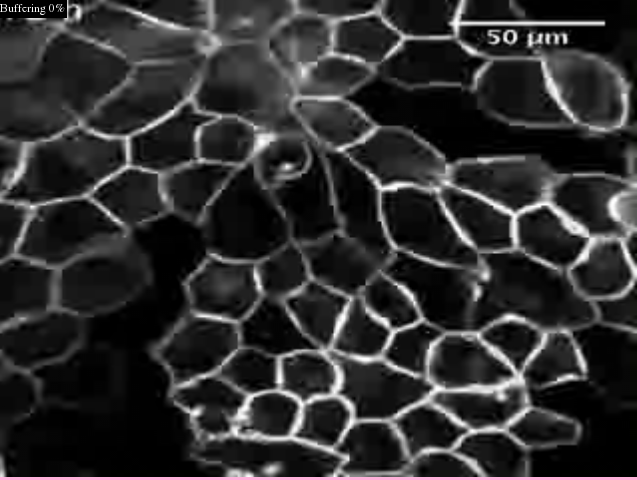
\includegraphics[height=5cm,width=5cm]{network_of_cells.png}
    \end{column}
    \begin{column}{0.8\textwidth}
        \begin{enumerate}
        \item < 1-| alert@1 > Tissue as a network of cells.
        \item < 2-| alert@2 > Cells as polygons.
        \item < 3-| alert@2 > Different cells \emph{shapes} are related to different kind of tissues\footnotemark.
        \end{enumerate}
    \end{column}
\end{columns}
\footcitetext{farhadifar2007influence}
\end{minipage}
\end{beamerboxesrounded}
}


%%%%%%%%%%%%%%%%%UNTIL HERE - CNS OCT-05-2015

\subsection{Classic model systems II}
\frame{\frametitle{Darwin finches, Cichlids, Orchids and Moths}
\setbeamercolor{uppercol}{fg=black,bg=white}
\setbeamercolor{lowercol}{fg=black,bg=white}
\begin{beamerboxesrounded}[upper=upperco,lower=lowercol,shadow=true]{}
\begin{columns}
\begin{column}{4cm}
\includegraphics<1>[width=2.5cm]{epiphysx.png}
\end{column}
\begin{column}{4cm}
\includegraphics<1>[width=2.5cm]{epiphysx.png}
\end{column}
\end{columns}
\end{beamerboxesrounded}
}

\subsection{Classic model systems III}
\frame{\frametitle{Darwin finches, Cichlids, Orchids and Moths}
\setbeamercolor{uppercol}{fg=black,bg=pink}
\setbeamercolor{lowercol}{fg=black,bg=pink}
\begin{beamerboxesrounded}[upper=upperco,lower=lowercol,shadow=true]{}
\begin{center}
\includegraphics<1>[height=4cm,width=9cm]{epiphysx.png}
\end{center}
\end{beamerboxesrounded}
}

\subsection{Classic model systems IV}
\frame{\frametitle{Darwin finches, Cichlids, Orchids and Moths}
\setbeamercolor{uppercol}{fg=black,bg=pink}
\setbeamercolor{lowercol}{fg=black,bg=pink}
\begin{beamerboxesrounded}[upper=upperco,lower=lowercol,shadow=true]{}
\vspace{-0.5 in}
\begin{center}
\includegraphics<1>[height=10cm,width=8cm,angle=90]{epiphysx.png}
\end{center}
\end{beamerboxesrounded}
}

\section{Questions}
\subsection{General questions}
\frame{\frametitle{Questions}
\begin{itemize}
\item < 1-| alert@1 > {\Large Do we need to invoke niche driven mechanisms to predict radiations and biodiversity patterns?} 
\item < 2-| alert@2 > {\Large Do quantitative genetics traits predict bimodal distributions in the absence of selection?}
\end{itemize}
}

\section{Radiations}

\subsection{Model I}
\frame{\frametitle{Genomes}
\setbeamercolor{uppercol}{fg=black,bg=white}
\setbeamercolor{lowercol}{fg=black,bg=white}
\begin{beamerboxesrounded}[upper=upperco,lower=lowercol,shadow=true]{}
\vspace{0.25 in}
\begin{center}
\hspace{-0.4 in}
\includegraphics[width=12cm]{epiphysx.png}
\end{center}
\end{beamerboxesrounded}
}

\subsection{Model II}
\frame{\frametitle{Genomes in a mating graph}
\setbeamercolor{uppercol}{fg=black,bg=white}
\setbeamercolor{lowercol}{fg=black,bg=white}
\begin{beamerboxesrounded}[upper=upperco,lower=lowercol,shadow=true]{}
\vspace{-0.25 in}
\begin{center}
\hspace{-0.95 in}
\includegraphics[width=14cm]{epiphysx.png}
\end{center}
\end{beamerboxesrounded}
}

\subsection{Model III}
\frame{\frametitle{Genomes in spatial landscapes}
\vspace{-0.25 in}
\begin{center}
\includegraphics<1>[height=7.5cm,width=7.5cm]{epiphysx.png}
\pause
\includegraphics<2>[height=7.5cm,width=7.5cm]{epiphysx.png}
\pause
\includegraphics<3>[height=7.5cm,width=7.5cm]{epiphysx.png}
\pause
\includegraphics<4>[height=7.5cm,width=7.5cm]{epiphysx.png}
\end{center}
}

\subsection{Radiations: theory}
\frame{\frametitle{Radiations: theory}
\setbeamercolor{uppercol}{fg=black,bg=white}
\setbeamercolor{lowercol}{fg=black,bg=white}
\begin{beamerboxesrounded}[upper=upperco,lower=lowercol,shadow=true]{}
\begin{center}
  \hspace{-0.15 in}
\includegraphics[width=8cm]{epiphysx.png}
\end{center}
\end{beamerboxesrounded}
}

\subsection{Radiations: data}
\frame{\frametitle{Radiations: data}
\setbeamercolor{uppercol}{fg=black,bg=white}
\setbeamercolor{lowercol}{fg=black,bg=white}
\begin{beamerboxesrounded}[upper=upperco,lower=lowercol,shadow=true]{}
\begin{center}
\hspace{0.5 in}
\includegraphics[width=10cm]{epiphysx.png}\footnotetext{{\Tiny Meli\'an, C. J. et. al
    (2010). Frequency-dependent selection predicts patterns of radiations and biodiversity, PLoS Comp. Biol., 6:e1000892.}}
\end{center}
\end{beamerboxesrounded}
}

\section{Networks}

%One oway is to simulate the spatio-temporal dynamics of thousands of individuals (simulation)
\subsection{Simulation}
\frame{\frametitle{Ecological, developmental, and evolutionary processes}
\setbeamercolor{uppercol}{fg=black,bg=pink}
\setbeamercolor{lowercol}{fg=black,bg=pink}
\begin{beamerboxesrounded}[upper=upperco,lower=lowercol,shadow=true]{}
\begin{minipage}[t]{6.1cm}
\hspace{4cm}\flashmovie[auto=0,loop=1,controlbar=1,engine=flv-player,width=6cm,height=6cm]{Animation.flv}
\end{minipage}
\end{beamerboxesrounded}
}

%4. Detailed cartoon of the model: describe the processes (fig)
\subsection{Description of the model}
\frame{\frametitle{Eco-devo-evo spatial dynamics}
\setbeamercolor{uppercol}{fg=black,bg=pink}
\setbeamercolor{lowercol}{fg=black,bg=pink}
\begin{beamerboxesrounded}[upper=upperco,lower=lowercol,shadow=true]{}
\begin{center}
\includegraphics<1>[height=6cm,width=8cm]{epiphysx.png}
\end{center}
\end{beamerboxesrounded}
}

\subsection{Bimodal}
\frame{\frametitle{Genotype-phenotype: theory}
\setbeamercolor{uppercol}{fg=black,bg=white}
\setbeamercolor{lowercol}{fg=black,bg=white}
\begin{beamerboxesrounded}[upper=upperco,lower=lowercol,shadow=true]{}
\begin{center}
  \hspace{-0.15 in}
\includegraphics[width=9cm]{epiphysx.png}
\end{center}
\end{beamerboxesrounded}
}

\subsection{Genotypes}
\frame{\frametitle{Genotype-phenotype: theory}
\setbeamercolor{uppercol}{fg=black,bg=white}
\setbeamercolor{lowercol}{fg=black,bg=white}
\begin{beamerboxesrounded}[upper=upperco,lower=lowercol,shadow=true]{}
\begin{center}
  \hspace{-0.15 in}
\includegraphics[width=9cm]{epiphysx.png}
\end{center}
\end{beamerboxesrounded}
}

\section{Outlook}

\subsection{Summary}
\frame{\frametitle{Outlook}
\setbeamercolor{uppercol}{fg=black,bg=white}
\setbeamercolor{lowercol}{fg=black,bg=white}
\begin{beamerboxesrounded}[upper=upperco,lower=lowercol,shadow=true]{}
\begin{enumerate}
\item < 1-| alert@1 > In addition to adaptive radiations driven by
  natural selection, just drift or negative frequency-dependent sexual
  selection may both predict some radiations.
\item < 2-| alert@2 > An incipient and testable framework to connect
  quantitative traits, speciation and biodiversity dynamics in
  ecological networks.
\end{enumerate}
\end{beamerboxesrounded}
}

\subsection{thankyou}
\frame{\frametitle{Thank you!}
\begin{itemize}
\item Scientists and technical staff at Wagner's group (IEU/UZH).
\item Scientists at Bastien's group (Unige).
\item SystemsX and SNSF.
\end{itemize}
}
%%%%%%%%%%%%%%%%%%%%%%%%%%%%%%%%%%%%%%%%%%%%%%%%%%%%%%%%%%%%%%%%%%%%%%%%%%%%%%%%%%%%%%%%%%
%%%%%%%%%%%%%%%%%%%%%%%%%%%%%% End Document %%%%%%%%%%%%%%%%%%%%%%%%%%%%%%%%%%%%%%%%%%%%%%
%%%%%%%%%%%%%%%%%%%%%%%%%%%%%%%%%%%%%%%%%%%%%%%%%%%%%%%%%%%%%%%%%%%%%%%%%%%%%%%%%%%%%%%%%%
\end{document}


\subsection{Distribution number of prey items per predator V}
\frame{\frametitle{All samplings with more than 2000 individuals sampled}
\begin{columns}
\begin{column}{10cm}
\vspace{-0.2 in}

\includegraphics[width=8cm]{epiphysx.png}
\end{column}
\end{columns}
}

\subsection{Strength of prey selection  (preliminary figure)}
\frame{\frametitle{Strength of prey selection in weakly-strongly connected individuals}
\begin{columns}
\begin{column}{12cm}
\vspace{-0.2 in}

\includegraphics[width=12cm]{epiphysx.png}
\end{column}
\end{columns}
}

\subsection{Strength of prey selection all individuals and sampled aggregated}
\frame{\frametitle{Strength of prey selection in weakly-strongly connected individuals (all)}
\vspace{-0.15 in}
\setbeamercolor{uppercol}{fg=black,bg=white}
\setbeamercolor{lowercol}{fg=black,bg=white}
\begin{beamerboxesrounded}[upper=upperco,lower=lowercol,shadow=true]{}
\begin{columns}
\begin{column}{10cm}

\includegraphics[width=9cm]{epiphysx.png}
\end{column}
\end{columns}
\end{beamerboxesrounded}
}

\subsection{Strength of prey selection and prey richness I}
\frame{\frametitle{Strength of prey selection and prey richness}
\vspace{-0.15 in}
\setbeamercolor{uppercol}{fg=black,bg=white}
\setbeamercolor{lowercol}{fg=black,bg=white}
\begin{beamerboxesrounded}[upper=upperco,lower=lowercol,shadow=true]{}
\begin{columns}
\begin{column}{10cm}

\includegraphics[width=6cm]{epiphysx.png}
\end{column}
\end{columns}
\end{beamerboxesrounded}
}

\subsection{Strength of prey selection and prey richness II}
\frame{\frametitle{Strength of prey selection and prey richness}
\vspace{-0.15 in}
\setbeamercolor{uppercol}{fg=black,bg=white}
\setbeamercolor{lowercol}{fg=black,bg=white}
\begin{beamerboxesrounded}[upper=upperco,lower=lowercol,shadow=true]{}
\begin{columns}
\begin{column}{10cm}

\includegraphics[width=6cm]{epiphysx.png}
\end{column}
\end{columns}
\end{beamerboxesrounded}
}



